\documentclass{article}

%\usepackage{corl_2017}
\usepackage[final]{corl_2017} % Uncomment for the camera-ready ``final'' version

\usepackage{amsmath,amsfonts,amssymb,subfigure,multirow,xcolor}
\usepackage[mathscr]{eucal}
%%%%%%%%%%%%%%%% macros %%%%%%%%%%%%%%%%%%

% refer to figures, sections in uniform way
\newcommand{\figref}[1]{{Figure~\ref{fig:#1}}}
\newcommand{\secref}[1]{{Section~\ref{sec:#1}}}
\newcommand{\propref}[1]{{Property~\ref{prop:#1}}}
\newcommand{\implref}[1]{{Implication~\ref{prop:#1}}}
\newcommand{\thmref}[1]{{Theorem~\ref{thm:#1}}}
\newcommand{\chref}[2]{\cite[Chapter~{#1}]{#2}}

\newcommand{\see}[1]{(see~#1)}
\newcommand{\cf}[1]{(cf.~#1)}
\newcommand{\etal}{\emph{et al.}}
\newcommand{\adhoc}{\emph{ad hoc.}}
\newcommand{\apriori}{\emph{a priori}}

\newcommand{\lft}{1}%{\text{left}}
\newcommand{\rght}{2}%{\text{right}}
\newcommand{\torque}{12}%{\text{torque}}
\newcommand{\touchdown}{\text{touchdown}}%{\text{torque}}
\newcommand{\liftoff}{\text{liftoff}}%{\text{torque}}

\newcommand{\Tstate}{v}
\newcommand{\Tinp}{w}
\newcommand{\param}{p}
\newcommand{\state}{x}
\newcommand{\run}{r}
\newcommand{\inp}{u}
\newcommand{\optstate}{\xi}
\newcommand{\optinp}{\mu}
\newcommand{\Param}{\e{P}}
\newcommand{\State}{\e{X}}
\newcommand{\Run}{\R}
\newcommand{\Inp}{\e{U}}
\newcommand{\ssState}{X}
\newcommand{\ssInp}{U}
\newcommand{\cost}{c}
\newcommand{\Ell}{\e{L}}
\newcommand{\val}{\nu}
\newcommand{\policy}{\pi}
%\newcommand{\policy}{\mu}
\newcommand{\flow}{\phi}
\newcommand{\D}{D}
\newcommand{\C}{C}
\newcommand{\T}{T}
\newcommand{\I}{I}
\newcommand{\PC}{PC}

\newcommand{\set}[1]{\left\{ #1 \right\}}
\newcommand{\paren}[1]{\left( #1 \right)}
\newcommand{\brak}[1]{\left[ #1 \right]}
\newcommand{\abs}[1]{\left| #1 \right|}
\newcommand{\norm}[1]{\left\| #1 \right\|}
\newcommand{\ip}[2]{\langle #1,#2 \rangle}
\newcommand{\pw}[1]{\left\{\begin{array}{ll} #1 \end{array}\right. }
\newcommand{\mat}[2]{\left[\begin{array}{#1} #2 \end{array}\right]}
\newcommand{\bd}{\partial}
\newcommand{\st}{\mid}
\newcommand{\td}[1]{\widetilde{#1}}
\newcommand{\ha}[1]{\widehat{#1}}
\newcommand{\eqn}[1]{\begin{equation*}\begin{aligned} #1 \end{aligned}\end{equation*}}
\newcommand{\eqnn}[1]{\begin{equation}\begin{aligned} #1 \end{aligned}\end{equation}}
\newcommand{\sm}{\setminus}
\newcommand{\conv}{\ast}
\newcommand{\into}{\rightarrow}
\newcommand{\goesto}{\rightarrow}
\newcommand{\goestoinp}{\xrightarrow{p}} 
\newcommand{\partialto}{\not\rightarrow}
\newcommand{\downto}{\downarrow}
\newcommand{\inc}{\hookrightarrow}

% inverse modeling 
\newcommand{\Mdl}{M}
\newcommand{\mdl}{m}
\newcommand{\out}{y}
\newcommand{\outd}{\des{\out}}
\newcommand{\Out}{Y}
\newcommand{\Nout}{n_{\out}}
\newcommand{\noise}{\veps}
\newcommand{\delay}{\tau}
\newcommand{\est}[1]{\td{#1}}
\newcommand{\inv}[1]{{#1}^{-1}}
\newcommand{\pinv}[1]{{#1}^{\dagger}}
\newcommand{\opt}[1]{{#1}^*}
\newcommand{\des}[1]{{#1}_d}
\newcommand{\xform}[1]{\ha{#1}}
\newcommand{\Xform}{\e{F}}
\newcommand{\nonlinear}{f}

\newcommand{\diffeo}{\Phi}
\newcommand{\Lie}{L}
\newcommand{\nhood}{X}
\newcommand{\mfold}{Z}
\newcommand{\err}{\varepsilon}
\newcommand{\contC}{C}
\newcommand{\contc}{c}

\newcommand{\Sn}{S_n}
\newcommand{\R}{\mathbb{R}}
\newcommand{\Z}{\mathbb{Z}}
\newcommand{\Hb}{\mathbb{H}}
\newcommand{\N}{\mathbb{N}}
\newcommand{\tr}{\top}
\newcommand{\TP}{\dagger}
\newcommand{\m}{\mathcal}
\newcommand{\e}{\mathscr}
\newcommand{\eps}{\epsilon}
\newcommand{\vphi}{\varphi}
\newcommand{\veps}{\varepsilon}
\newcommand{\ones}{\mathds{1}}
\newcommand{\id}{\operatorname{id}}
\newcommand{\suth}{\ \text{s.t.}\ }
\newcommand{\rk}{\operatorname{rank}}
\newcommand{\spn}{\operatorname{span}}
\newcommand{\diag}{\operatorname{diag}}
\newcommand{\Int}[1]{\operatorname{Int}#1}
\newcommand{\pset}[1]{2^{#1}}
\newcommand{\cl}[1]{\operatorname{cl}\paren{#1}}
\newcommand{\sgn}{\operatorname{sign}}
\newcommand{\spec}{\operatorname{spec}}

\newtheorem{proposition}{Proposition}
\newtheorem{definition}{Definition}
\newtheorem{theorem}{Theorem}
\newtheorem{corollary}{Corollary}
\newtheorem{lemma}{Lemma}
\newtheorem{claim}{Claim}
\newtheorem{assumption}{Assumption}
\newtheorem{remark}{Remark}
\newtheorem{property}{Property}
\newtheorem{implication}{Implication}
\newtheorem{example}{Example}

%\newcommand{property}[3]{\noindent\textbf{Property~#1 (#2).} #3}
%\newcommand{prop}[1]{\noindent\textbf{Property.} #3}

\newcommand{\defn}[1]{\begin{definition} #1 \end{definition}}
\newcommand{\defna}[2]{\begin{definition}[#1] #2 \end{definition}}
\newcommand{\rem}[1]{\begin{remark} #1 \end{remark}}
\newcommand{\remna}[2]{\begin{remark}[#1] #2 \end{remark}}
\newcommand{\assump}[1]{\begin{assumption} #1 \end{assumption}}
\newcommand{\assumpn}[2]{\begin{assumption}[#1] #2 \end{assumption}}
\newcommand{\lem}[1]{\begin{lemma} #1 \end{lemma}}
\newcommand{\clm}[1]{\begin{claim} #1 \end{claim}}
\newcommand{\ex}[1]{\begin{example} #1 \end{example}}
\newcommand{\exn}[2]{\begin{example}\emph{(#1)} #2 \end{example}}
\newcommand{\thm}[1]{\begin{theorem} #1 \end{theorem}}
\newcommand{\prop}[1]{\begin{proposition} #1 \end{proposition}}
\newcommand{\propn}[2]{\begin{proposition}[#1] #2 \end{proposition}}
\newcommand{\pf}[1]{\begin{proof} #1 \end{proof}}
\newcommand{\cor}[1]{\begin{corollary} #1 \end{corollary}}


\newcommand{\asmpdiff}{Assump.~\ref{asmp:diff} (differentiable vector field and reset map)}
\newcommand{\asmpanalytic}{Assump.~\ref{asmp:analytic} (analytic dynamics)}
\newcommand{\asmpmass}{Assump.~\ref{asmp:mass} (invertible mass matrix)}
\newcommand{\asmpcomplete}{Assump.~\ref{asmp:complete} (complete configuration space)}
\newcommand{\asmpindep}{Assump.~\ref{asmp:indep} (independent constraints)}
\newcommand{\asmplipschitz}{Assump.~\ref{asmp:lipschitz} (Lipschitz effort)}
\newcommand{\asmporth}{Assump.~\ref{asmp:orth} (orthogonal constraints)}
\newcommand{\asmpdecoupled}{Assump.~\ref{asmp:decoupled} (limbs decoupled through body)}
\newcommand{\asmptrj}{Assump.~\ref{asmp:trj} (admissible trajectories)}
\newcommand{\remorth}{Remark~\ref{rem:orth} (inertial decoupling)}
\newcommand{\remmass}{Remark~\ref{rem:mass} (invertible mass matrix)}
\newcommand{\remindep}{Remark~\ref{rem:indep} (independent constraints)}
\newcommand{\remcomplete}{Remark~\ref{rem:complete} (complete configuration space)}
\newcommand{\remlipschitz}{Remark~\ref{rem:lipschitz} (Lipschitz effort)}
\newcommand{\remseq}{Remark~\ref{rem:seq} (contact mode sequence)}
\newcommand{\remtrj}{Remark~\ref{rem:trj} (admissible trajectories)}
\newcommand{\remadact}{Remark~\ref{rem:adact}}
\newcommand{\defcontact}{Def.~\ref{def:contact} (contact modes)}
\newcommand{\defipnorm}{Def.~\ref{def:ipnorm} (inner products and norms)}
\newcommand{\defact}{Def.~\ref{def:act} (constraint activation/deactivation)}
\newcommand{\defadact}{Def.~\ref{def:adact} (admissible constraint activation/deactivation)}
\newcommand{\deftrj}{Def.~\ref{def:trj} (admissible trajectory)}
\newcommand{\defseq}{Def.~\ref{def:seq} (contact mode sequence)}
\newcommand{\lemflow}{Lem.~\ref{lem:flow} (existence and uniqueness)}
\newcommand{\lemdiffi}{Lem.~\ref{lem:diffi} (differentiability within contact mode sequences)}
\newcommand{\lemcont}{Lem.~\ref{lem:cont} (continuity across contact mode sequences)}
\newcommand{\thmdiff}{Thm.~\ref{thm:diff} (differentiability through intermittent contact)}
\newcommand{\thmdiffb}{Thm.~\ref{thm:diffb} (piecewise differentiability across contact mode sequences)}
\newcommand{\thmdiffba}{Thm.~\ref{thm:diffb:a} (piecewise differentiability across contact mode sequences for constraint activation)}
\newcommand{\thmdiffbd}{Thm.~\ref{thm:diffb:d} (piecewise differentiability across contact mode sequences for constraint deactivation)}



\usepackage{todonotes}
\let\todon\todo
\newcommand{\tbd}[2][]{\todon[color=red!40,size=\scriptsize,#1]{TODO: #2}}
\newcommand{\sam}[2][]{\todon[color=blue!40,size=\scriptsize,#1]{Sam: #2}}
\newcommand{\bora}[2][]{\todon[color=orange!40,size=\scriptsize,#1]{Bora: #2}}

\title{Regularity of optimal value and policy functions for mechanical systems subject to unilateral constraints}

\author{
  Bora Banjanin, Samuel A. Burden\\
  Department of Electrical Engineering\\
  University of Washington, Seattle, WA, USA\\
  \texttt{borab,sburden@uw.edu} \\
  %% examples of more authors
  %% \And
  %% Coauthor \\
  %% Affiliation \\
  %% Address \\
  %% \texttt{email} \\
  %% \AND
  %% Coauthor \\
  %% Affiliation \\
  %% Address \\
  %% \texttt{email} \\
  %% \And
  %% Coauthor \\
  %% Affiliation \\
  %% Address \\
  %% \texttt{email} \\
  %% \And
  %% Coauthor \\
  %% Affiliation \\
  %% Address \\
  %% \texttt{email} \\
}


\begin{document}
\maketitle

%===============================================================================

\begin{abstract}
State--of--the--art approaches to reinforcement learning for contact--rich robot dynamics use smooth approximations of value and policy functions and gradient--based algorithms for improving approximator parameters. 
Unfortunately, the dynamics of mechanical systems subject to unilateral constraints---i.e. robot locomotion and manipulation---are generally nonsmooth. % (discontinuous or piecewise--differentiable).
We show that value and policy functions generally inherit regularity properties like (non)smoothness from the underlying system's dynamics, and demonstrate this effect in a simple mechanical system.
We conclude with a discussion of implications for the use of smooth function approximators and gradient--based algorithms for contact--rich robot dynamics arising in locomotion and manipulation. %optimal control of mechanical systems subject to unilateral constraints.
\end{abstract}

\keywords{%
locomotion, 
manipulation, 
piecewise--differentiability
} 

\section{Introduction and background on optimal value and policy functions}
\label{sec:value}

Consider minimization of the \emph{cost function} $c:\State\times\Inp\into\R$ with respect to an \emph{input} $\inp\in \Inp$:
\eqnn{\label{eq:min}
\val(\state) = \min_{\inp\in \Inp} \cost(\state,\inp);
}
so long as $\State$ and $\Inp$ are compact and $\cost$ is continuous,
the function $\nu:\State\into \R$ indicated in~\eqref{eq:min}, termed the \emph{optimal value function}, is well--defined.
%
We let $\policy:\State\into \Inp$ denote an \emph{optimal policy} for~\eqref{eq:min}, i.e.
\eqnn{\label{eq:argmin}
\forall \state\in \State : \policy(\state) & \in \arg\min_{\inp\in \Inp} \cost(\state,\inp)\\ 
}
or, equivalently,
\eqnn{\label{eq:value}
\forall \state\in \State : \val(\state) & = \cost(\state,\policy(\state)).
}

In this paper we study how regularity properties (continuity, differentiability) of the cost function ($c$) relate to regularity properties of optimal value ($\val$) and policy ($\policy$) functions,
and apply these results to optimal control problems involving contact--rich robot dynamics.

\paragraph{Organization:}
the remainder of this section concerns regularity properties of optimal value and policy functions;
\secref{sys} describes a class of models for contact--rich robot dynamics;
\secref{opt} presents optimal value and policy functions in a simple mechanical system;
\secref{disc} discusses generality and implications of these results.


\subsection{Discontinuous cost functions}
\label{sec:value:nc}
If the cost 
($\cost:\State\times\Inp\into\R$) is discontinuous with respect to its first argument, then the optimal policy 
($\policy:\State\into\Inp$) and value 
($\val:\State\into\R$) are generally discontinuous as well.
This observation is clear in the trivial case that the cost only depends on its first argument, but manifests more generally.


\subsection{Continuously--differentiable cost functions}
\label{sec:value:c}

This section contains straightforward calculations based on standard results in classical (smooth) Calculus and nonlinear programming; it is provided primarily as a rehearsal for the more general setting considered in the subsequent section.

If $\cost$ is continuously--differentiable, denoted $\cost\in\C^1(\State\times \Inp,\R)$ or simply $\cost\in\C^1$, then necessarily~\cite[Ch.~1.1.1]{Polak1997-xd}
\eqnn{\label{eq:c:nec_}
\D_2 \cost(\state,\policy(\state)) = 0.
}

If $\cost$ is two times continuously--differentiable (denoted $\cost\in\C^2$) and the second--order sufficient condition~\cite[Ch.~1.1.2]{Polak1997-xd} for strict local optimality for~\eqref{eq:min} is satisfied at $\policy(\state)\in\Inp$,
\eqnn{\label{eq:c:suf_}
\D_2^2 \cost(\state,\policy(\state)) > 0,
}
then the $\C^1$ Implicit Function Theorem (IFT)~\citep[Thm.~C.40]{Lee2012-mb} can be applied to~\eqref{eq:value} to choose $\policy$ as a $\C^1$ function near $\state$.
Note that IFT specifically required the invertibility tacit in~\eqref{eq:c:suf_}: 
\eqnn{\label{eq:c:stab}
\text{the linear function}\ \D_2^2 \cost(\state,\policy(\state)):\T_\inp\Inp\into\T_\inp\Inp\ \text{is invertible}.
}

If~\eqref{eq:c:nec_} and~\eqref{eq:c:suf_} are satisfied, then 
applying the $\C^1$ Chain Rule~\citep[Prop.~C.3]{Lee2012-mb} to~\eqref{eq:c:nec_} yields

\eqnn{\label{eq:c:Dpolicy}
\D\policy(\state) & = - \D_2^2 \cost(\state,\policy(\state))^{-1}\paren{\D_{12}\cost(\state,\policy(\state))},
}
and applying the $\C^1$ Chain Rule to~\eqref{eq:value} yields
\eqnn{\label{eq:c:Dval}
\D\val(\state) & = \D_\state \cost(\state,\policy(\state)) %\\
& = \D_1 \cost(\state,\policy(\state)) + \D_2 \cost(\state,\policy(\state)) \D\policy(\state),
}
whence we obtain derivatives of the optimal value and policy functions in terms of derivatives of the cost function.

We conclude that if the cost function is two times continuously--differentiable ($\cost\in\C^2$) and first--order necessary~\eqref{eq:c:nec_} and second--order sufficient~\eqref{eq:c:suf_},~\eqref{eq:c:stab} conditions for optimality and stability of solutions to~\eqref{eq:min} are satisfied at $\inp = \policy(\state)$, then the optimal policy and value functions are continuously--differentiable at $\state$ ($\policy,\val\in\C^1$) and their derivatives at $\state$ can be computed using~\eqref{eq:c:Dpolicy},~\eqref{eq:c:Dval}.

\prop{\label{prop:c}
If $\cost\in\C^2(\State\times\Inp,\R)$ satisfies~\eqref{eq:c:nec_},~\eqref{eq:c:suf_}, and~\eqref{eq:c:stab} at $(\optstate,\optinp)\in\State\times\Inp$,
then 
there exist neighborhoods
$\ssState\subset\State$ of $\optstate$ 
and
$\ssInp\subset\Inp$ of $\optinp$ 
and
$\policy\in\C^1(\ssState,\ssInp)$ 
such that $\policy(\optstate) = \optinp$ and
\eqnn{
\forall \state\in\ssState 
: 
\policy(\state)\ \text{is the unique minimizer for}\ \val(x) = \min_{\inp\in\ssInp} \cost(\state,\inp);
}
the derivative of $\policy$ is given by~\eqref{eq:c:Dpolicy}, 
and
the derivative of $\val$ is given by~\eqref{eq:c:Dval}.
}


\subsection{Piecewise--differentiable cost functions}
\label{sec:value:pc}

If $\cost$ is piecewise--differentiable,%
\footnote{We use the notion of piecewise--differentiability from~\cite[Ch.~4.1]{Scholtes2012-la}: a function is piecewise--differentiable if it is everywhere locally a continuous selection of a finite number of continuously--differentiable functions.}
denoted $\cost\in\PC^1(\State\times \Inp,\R)$ or simply $\cost\in\PC^1$, then necessarily%
\eqnn{\label{eq:pc:nec}
\forall \Tinp\in\T_\inp\Inp 
: 
\D_2 \cost(\state,\policy(\state);\Tinp) \ge 0.
}
Here and below, 
$\D_2 \cost(\state,\policy(\state)):\T_\inp\Inp\into\R$ 
denotes a continuous and piecewise--linear first--order approximation termed the \emph{Bouligand} (or \emph{B--})derivative~\citep[Ch.~3]{Scholtes2012-la} that exists by virtue of the cost being $\PC^1$~\citep[Lem.~4.1.3]{Scholtes2012-la}; 
$\D_2 \cost(\state,\policy(\state);\Tinp)$ 
denotes the evaluation of
$\D_2 \cost(\state,\policy(\state))$
at $\Tinp\in\T_\inp\Inp$.

If 
$\cost$ is two times piecewise--differentiable (denoted $\cost\in\PC^2$), 
and if a sufficient condition~\cite[Thm.~1]{Chaney1988-zq} for strict local optimality%
%\footnote{Unlike~\eqref{eq:c:suf}, 
%the set $\set{\Tinp\in\T_\inp\Inp \st \Tinp\ne 0,\ \D_2\cost(\state,\policy(\state);\Tinp) = 0}$ is not necessarily $\T_\inp\Inp\sm\set{0}$ 
%since $\D_2\cost(\state,\policy(\state)):\T_\inp\Inp\into\R$ is not necessarily the zero operator; 
%consider $\cost(\state,\policy(\state)) = \abs{\inp}$ at $\inp=0$.}
%
~for~\eqref{eq:min} is satisfied at $\policy(\state)\in\Inp$,
\eqnn{\label{eq:pc:suf}
\forall \Tinp\in \set{\Tinp\in\T_\inp\Inp \st \Tinp\ne 0,\ \D_2\cost(\state,\policy(\state);\Tinp) = 0}
:
\D_2^2 \cost(\state,\policy(\state);\Tinp,\Tinp) > 0,
}
and if%
%\footnote{Unlike the continuously--differentiable case, where~\eqref{eq:c:suf} implies \eqref{eq:c:stab}, in the piecewise--differentiable case~\eqref{eq:pc:suf} does not necessarily imply~\eqref{eq:pc:stab}.}
\eqnn{\label{eq:pc:stab}
\text{the piecewise--linear function}\ \D_2^2 \cost(\state,\policy(\state)):\T_\inp\Inp\into\T_\inp\Inp\ \text{is invertible},
}
then a $\PC^1$ Implicit Function Theorem can be applied to choose $\policy$ as a $\PC^1$ function near $\state$~\citep[Cor.~3.4]{Robinson1991-xg}.%
\footnote{This Implicit Function Theorem requires $\D_2\cost$ be \emph{strongly} B--differentiable; the costs considered below are not generally strongly B--differentiable, but they are generally $\PC^r$--equivalent to strongly B--differentiable functions~\cite[Thm.~3.1]{Kuntz1994-qf}, whence~\cite[Cor.~3.4]{Robinson1991-xg} can be applied indirectly.} Applying the $\PC^1$ Chain Rule~\citep[Thm.~3.1.1]{Scholtes2012-la} to~\eqref{eq:pc:nec} yields~\cf{~\cite[\S~3]{Robinson1991-xg}}
\eqnn{\label{eq:pc:Dpolicy}
\forall \Tstate\in\T_\state\State : \D\policy(\state;\Tstate) & = - \D_2^2 \cost(\state,\policy(\state))^{-1}\paren{\D_{12}\cost(\state,\policy(\state);\Tstate)},
}
and applying the $\PC^1$ Chain Rule to~\eqref{eq:value} yields
\eqnn{\label{eq:pc:Dval}
\forall \Tstate\in\T_\state\State : \D\val(\state;\Tstate) & = \D_\state \cost(\state,\policy(\state);v) %\\
& = \D_1 \cost(\state,\policy(\state);\Tstate) + \D_2 \cost(\state,\policy(\state);\D\policy(\state;\Tstate)),
}
whence we obtain B--derivatives of the optimal value and policy functions in terms of B--derivatives of the cost function.

We conclude that if the cost function is two times piecewise--differentiable ($\cost\in\PC^2$) and first--order necessary~\eqref{eq:pc:nec} and second--order sufficient~\eqref{eq:pc:suf},~\eqref{eq:pc:stab} conditions for optimality and stability of solutions to~\eqref{eq:min} are satisfied at $\inp = \policy(\state)$, then the optimal policy and value functions are piecewise--differentiable at $\state$ ($\policy,\val\in\PC^1$) and their B--derivatives at $\state$ can be computed using~\eqref{eq:pc:Dpolicy},~\eqref{eq:pc:Dval}.

\prop{\label{prop:pc}
If 
$\cost\in\PC^2(\State\times\Inp,\R)$ satisfies~\eqref{eq:pc:nec},~\eqref{eq:pc:suf}, and~\eqref{eq:pc:stab} at $(\optstate,\optinp)\in\State\times\Inp$,
then 
there exist neighborhoods
$\ssState\subset\State$ of $\optstate$ 
and
$\ssInp\subset\Inp$ of $\optinp$ 
and
$\policy\in\PC^1(\ssState,\ssInp)$ 
such that $\policy(\optstate) = \optinp$ and
\eqnn{
\forall \state\in\ssState 
: 
\policy(\state)\ \text{is the unique minimizer for}\ \val(x) = \min_{\inp\in\ssInp} \cost(\state,\inp);
}
the B--derivative of $\policy$ is given by~\eqref{eq:pc:Dpolicy}, 
and
the B--derivative of $\val$ is given by~\eqref{eq:pc:Dval}.
}

\subsection{Conclusions regarding regularity of optimal value and policy functions}
The results in Sections~\ref{sec:value:nc},~\ref{sec:value:c}, and~\ref{sec:value:pc} suggest that we should generally expect regularity of optimal value and policy functions to match that of the cost function:  they should be discontinuous when the cost is discontinuous, or piecewise--differentiable when the cost is piecewise--differentiable.
In~\secref{opt} we provide instances of the class of models described in~\secref{sys} that exhibit these effects. 

\begin{figure}

\centering
\subfigure[\emph{touchdown} maneuver illustration]{
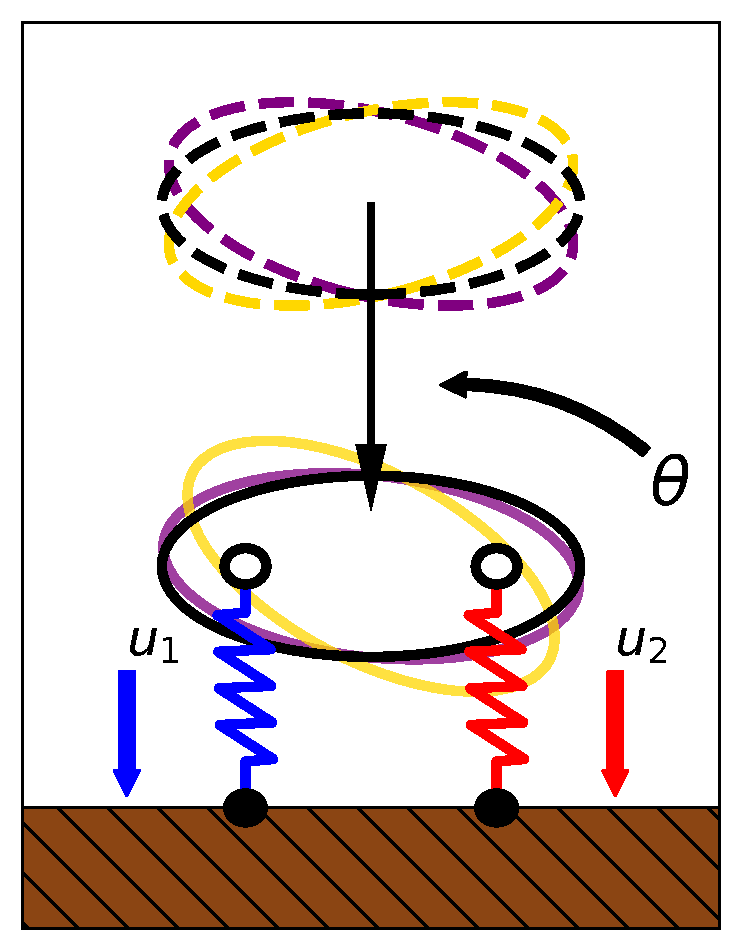
\includegraphics[width=.35\textwidth]{1a.pdf}\quad
}
\subfigure[\emph{liftoff} maneuver illustration]{
\quad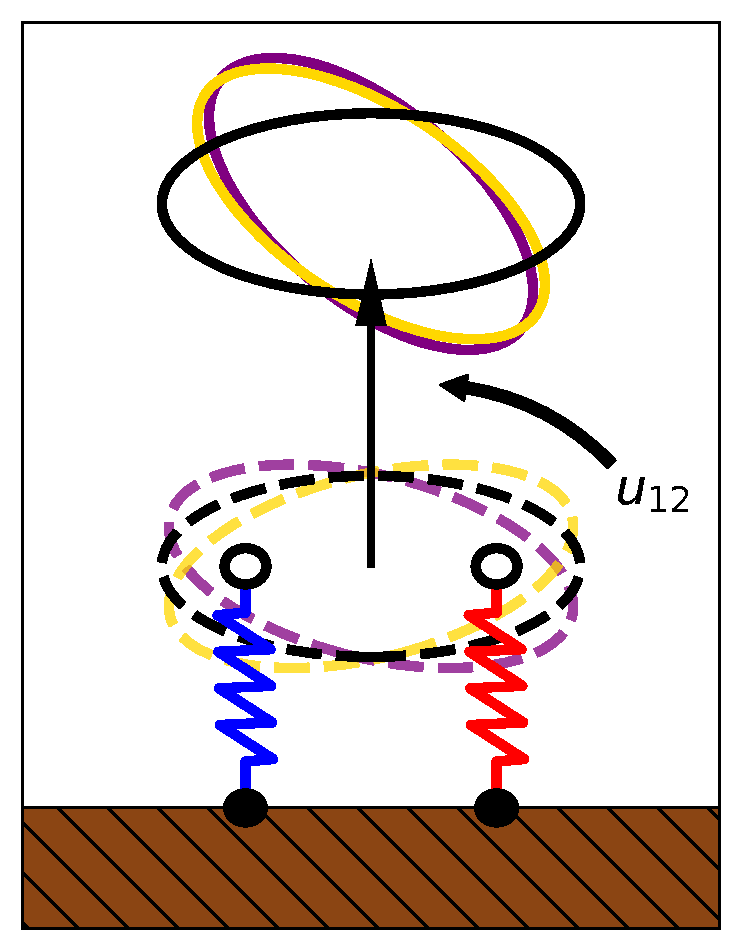
\includegraphics[width=.35\textwidth]{1b.pdf}
}

\subfigure[touchdown trajectory outcomes]{
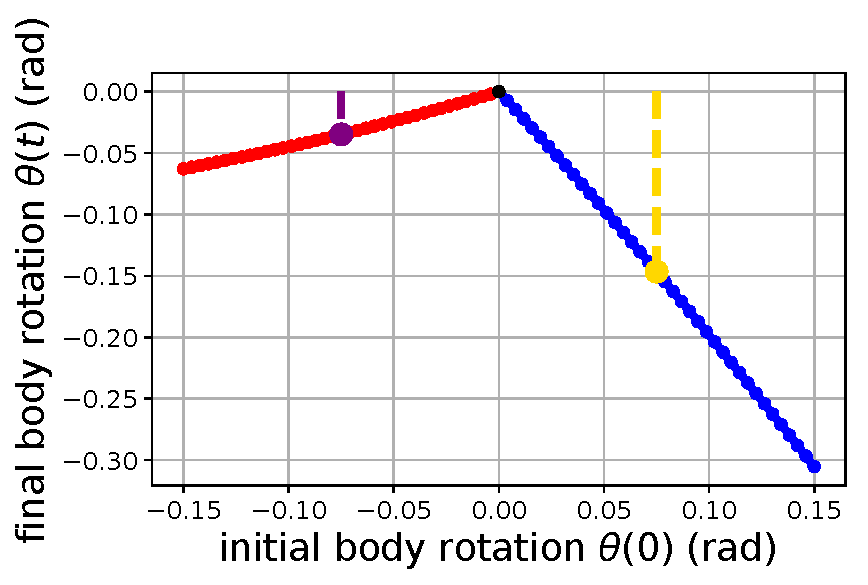
\includegraphics[width=.48\textwidth]{1c.pdf}
}
\subfigure[liftoff trajectory outcomes]{
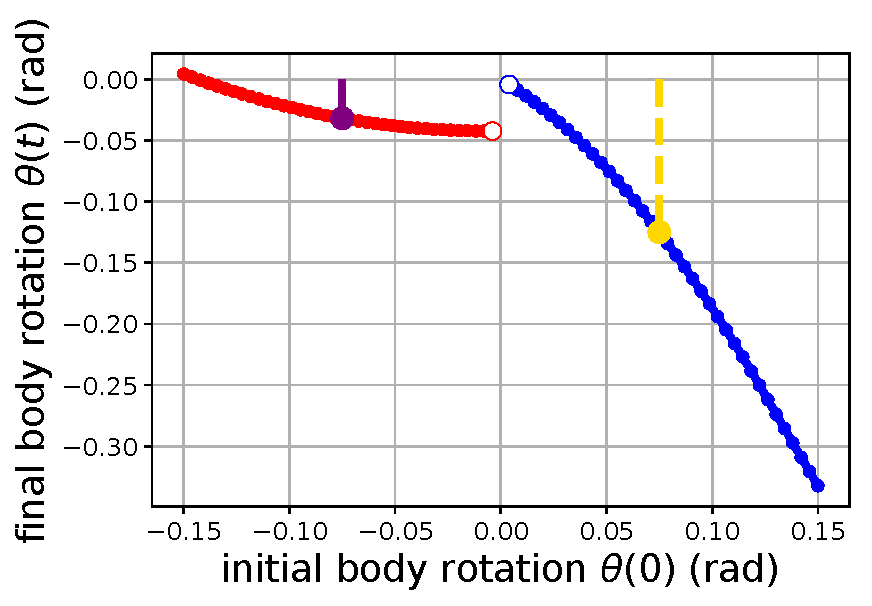
\includegraphics[width=.48\textwidth]{1d.pdf}
}

\subfigure[touchdown value]{
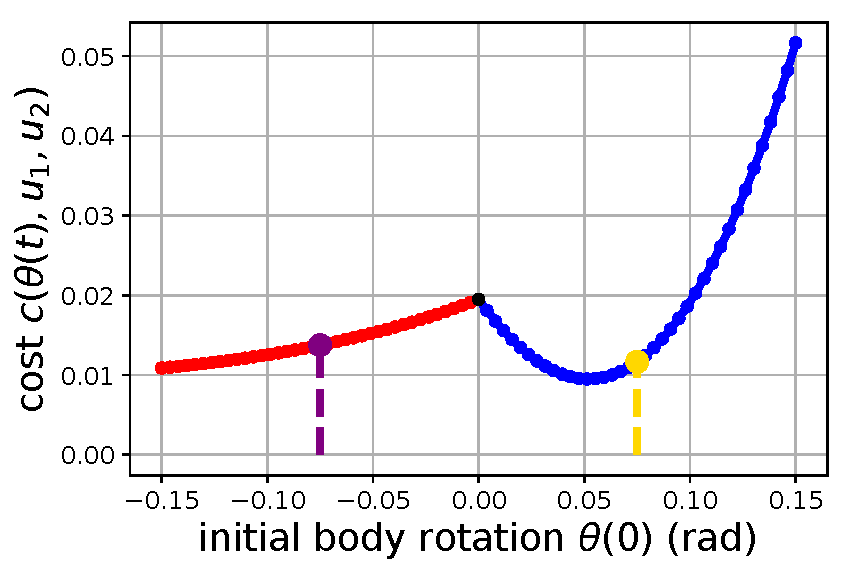
\includegraphics[width=.48\textwidth]{1e.pdf}
}
\subfigure[liftoff value]{
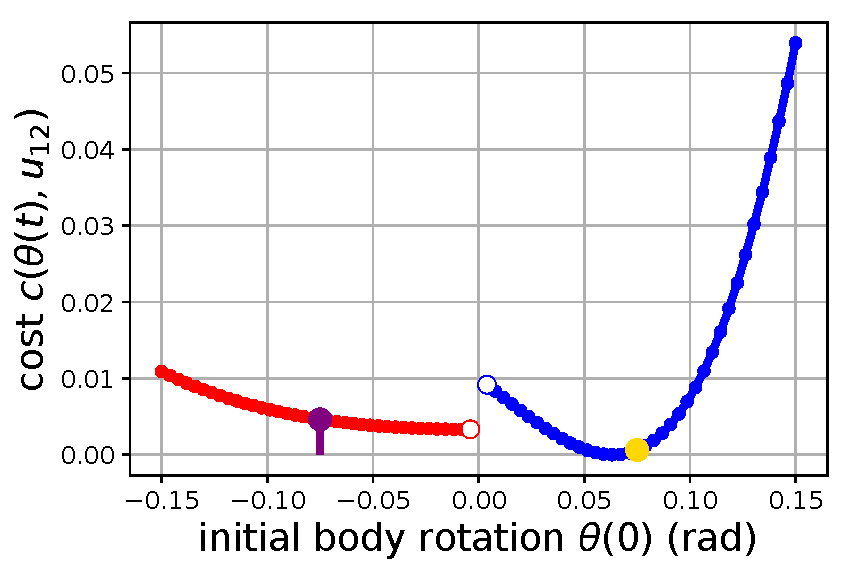
\includegraphics[width=.48\textwidth]{1f.pdf}
}

\caption{\label{fig:mdls}
\emph{Piecewise--differentiable and discontinuous trajectory outcomes in saggital--plane biped.} 
(a,b) Illustration of two maneuvers---\emph{touchdown} and \emph{liftoff}---performed under non--optimal policies that exert different forces %in each \emph{contact mode}~\cf{Def.~\ref{def:contact}} 
depending on which feet are in contact with the ground.
%
In the \emph{touchdown} maneuver, feet are initially off the ground and trajectories terminate when the body height reaches nadir;
in the \emph{liftoff} maneuver, feet are initially on the ground and trajectories terminate when the body height reaches apex.
(c,d) Trajectory outcomes (final body angle $\theta(t)$) as a function of initial body angle $\theta(0)$.
(e,f) Performance of trajectories as measured by the cost functions in~\eqref{eq:touchdown:cost},~\eqref{eq:liftoff:cost}.
Dashed colored vertical lines on (c--f) indicate corresponding colored outcomes on (a,b).
}
\end{figure}


%==========

\section{Mechanical systems subject to unilateral constraints}
\label{sec:sys}

\begin{figure}

\centering
\subfigure[touchdown contact modes]{
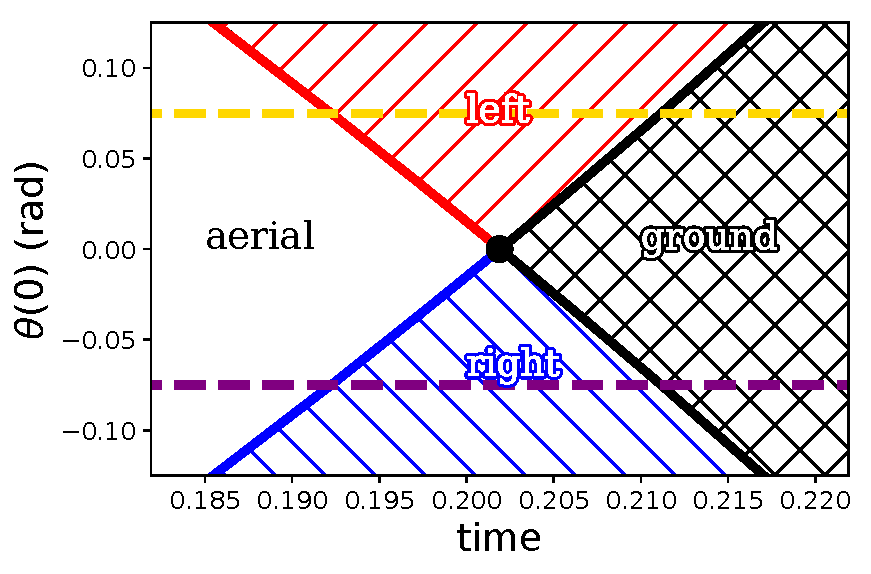
\includegraphics[width=.48\textwidth]{2a.pdf}
}
\subfigure[liftoff contact modes]{
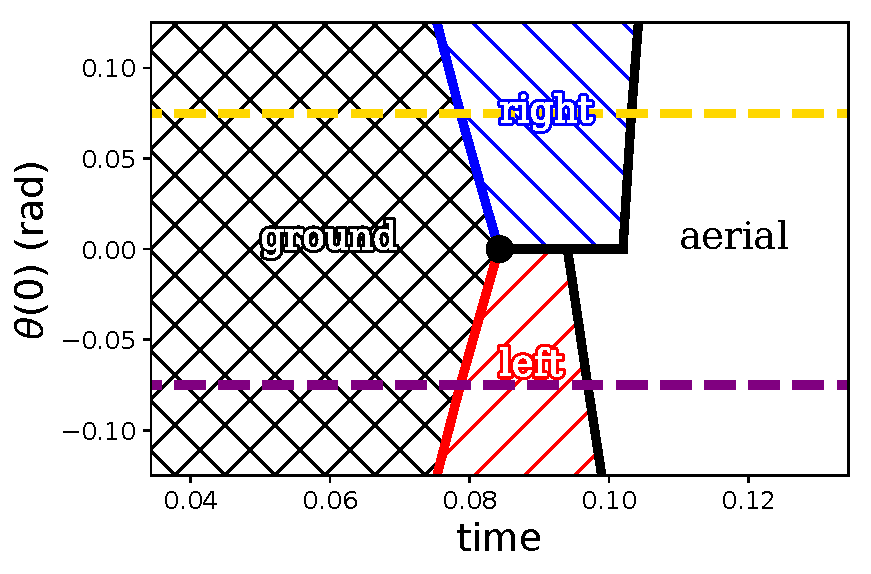
\includegraphics[width=.48\textwidth]{2b.pdf}
}

\caption{\label{fig:contact}
\emph{Contact modes for touchdown and liftoff maneuvers.}
The saggital--plane biped illustrated in~\figref{mdls}(a,b) can be in one of four \emph{contact modes} corresponding to which subset $J\subset\set{1,2}$ of the (two) limbs are in contact with the ground; each subset yields different dynamics in~\eqref{eq:dyn}.
(a,b) System contact mode 
at each time $t$ 
for a given initial body rotation $\theta(0)$;
the body torque is zero and the leg forces are different in mode \emph{left} ($\set{1}$) and \emph{right} ($\set{2}$) than in \emph{aerial} ($\emptyset$) or ground ($\set{1,2}$).
Dashed colored horizontal lines indicate corresponding colored trajectories in~\figref{mdls}.
%\\
The increase in force 
during the transition to modes \emph{left} and \emph{right}
in (b) 
changes the ground reaction force discontinuously, delaying liftoff %for the corresponding foot;
%this causes the 
and causing
discontinuous trajectory outcomes in~\figref{mdls}(d).
%
%The domain evolution for the down (a) and up (b) systems with respect to time and initial rotational angle. The dashed lines correspond to the two reference trajectories from Figure 1.
}
\end{figure}

In this section, we formalize a class of models relevant for contact--rich dynamics in robot locomotion and manipulation as \emph{mechanical systems subject to unilateral constraints} and apply results from the preceding section to optimal control problems involving these models.

\subsection{Dynamics}
\label{sec:dyn}
Consider the dynamics of a mechanical system with configuration coordinates $q\in Q=\R^d$ subject to 
unilateral constraints $a(q) \ge 0$ 
specified by a differentiable function 
$a : Q\into \R^n$
where $d,n\in\N$ are finite.
We are primarily interested in systems with $n > 1$ constraints,  
whence we regard the inequality $a(q) \ge 0$ as being enforced componentwise.

Given any $J\subset\set{1,\dots,n}$, 
and letting $\abs{J}$ denote the number of elements in the set $J$,
we let 
$a_J : Q \into \R^{\abs{J}}$ 
denote the function obtained by selecting the component functions of $a$ indexed by $J$, 
and we regard the equality $a_J(q) = 0$ as being enforced componentwise.

It is well--known~\cf{~\cite[Sec.~3]{Ballard2000-ui} or \cite[Sec.~2.4,~2.5]{Johnson2016-nh}}
that, with
$J = \set{j\in\set{1,\dots,n} : a_j(q) = 0}$ 
denoting the \emph{contact mode},
the system's dynamics take the form
\begin{subequations}\label{eq:dyn}
\begin{align}
  M(q)\ddot{q} & = f_J(q,\dot{q},\inp) + c(q,\dot{q})\dot{q} + Da_J(q)^\tr \lambda_J(q,\dot{q},u),\label{eq:dyn:cont}\\
  \dot{q}^+ & = \Delta_J(q,\dot{q}^-),\label{eq:dyn:disc}
\end{align}
\end{subequations}
%}
where
%M
$M : Q \into \R^{d\times d}$
specifies the mass matrix for the mechanical system in the $q$ coordinates,
%f
$f_J : TQ \into \R^d$ 
is termed the \emph{effort map}~\cite{Ballard2000-ui}
and specifies%
\footnote{We let $TQ = \R^d\times\R^d$ denote the \emph{tangent bundle} of the configuration space $Q$; an element $(q,\dot{q})\in TQ$ can be regarded as a pair containing generalized configurations $q\in\R^d$ and velocities $\dot{q}\in\R^d$; we write $\dot{q}\in T_q Q$.}
the internal and applied
forces, 
%u
$\inp\in\Inp$ is an external input,
%c
$c : TQ \into \R^{d\times d}$ 
denotes the \emph{Coriolis matrix} 
determined by $M$,
%Da
$Da_J : Q \into \R^{\abs{J}\times d}$ 
denotes the (Jacobian) derivative of the constraint function $a_J$ with respect to the coordinates,
%\lambda
$\lambda_J : TQ \into \R^{\abs{J}}$ 
denotes the reaction forces generated in contact mode $J$ to enforce $a_J(q) \ge 0$,
%\eqnn{
%\lambda_J(q) = \paren{Da_J(q) M(q)^{-1} Da_J(q)^\tr}^{-1},
%}
%\Delta
$\Delta_J : TQ \into \R^{d\times d}$ 
specifies the collision restitution law that instantaneously resets velocities to ensure compatibility with the constraint $a_J(q) = 0$,
%\eqnn{
%\dot{q}^+ = \Delta_J(q,\dot{q}^-) = \I - (1+\gamma(q,\dot{q}^-)) P_J(q)\dot{q}^-,
%}
%where 
%$\I$ is the $(d\times d)$ identity matrix,
%$\gamma : TQ\into[0,\infty)$ specifies the \emph{coefficient of restitution},
%$P_J:Q\into \R^{d\times d}$ is the projection onto the constraint surface,
%\eqnn{
%P_J = M^{-1} Da_J^\tr \paren{Da_J M^{-1} Da_J^\tr}^{-1} Da_J,
%}
%
and
$\dot{q}^+$ (resp. $\dot{q}^-$) denotes the right-- (resp. left--)handed limits of the velocity with respect to time.
%

\subsection{Regularity of dynamics}
\label{sec:reg:dyn}
The seemingly benign equations in~\eqref{eq:dyn} 
can yield dynamics with a range of regularity properties.
This issue has been thoroughly investigated elsewhere~\cite{Pace2017-tt, Pace2017-ph, Ballard2000-ui};
here we focus specifically on how design choices in a robot's \emph{mechanical} and \emph{control} systems affect regularity of its dynamics.

In what follows, we will frequently refer to the concept of a control system's \emph{flow}, so we briefly review the concept before proceeding.
Given a control system (e.g.~\eqref{eq:dyn} or~\eqref{eq:c:dyn}) with state space $\State$ and input space $\Inp$, 
a \emph{flow} is a function
$\flow:[0,t]\times\State\times\Inp^{[0,t]}\into\State$
such that for all initial states $\state\in\State$ and inputs $\paren{\inp:[0,t]\into\Inp}\in\Inp^{[0,t]}$,
the function 
$\flow^{x,u}:[0,t]\into\State$ 
defined for all $s\in[0,t]$ by 
$\flow^{x,u}(s) = \flow(s,x,u)$
is a trajectory for the control system.
Intuitively, the flow ``bundles'' all trajectories into a single function.
Mathematically, the flow is useful for studying how trajectories vary with respect to initial states and inputs.
So long as trajectories exist and are unique for every $\state\in\State$ and $\inp\in\Inp^{[0,t]}$, the flow is a well--defined function.

It is common to assume that the functions in~\eqref{eq:dyn} are continuously--differentiable ($M, f, a, \gamma\in\C^r$); however, as illustrated by~\cite[Ex.~2]{Ballard2000-ui}, this assumption alone does not ensure existence or uniqueness of trajectories.
This case contrasts starkly with that of classical 
%(non--hybrid) 
control systems, where the equation
\eqnn{\label{eq:c:dyn}
\dot{x} = F(x,u)
}
yields unique trajectories whose regularity matches the vector field's:
%if $F$ is Lipschitz continuous,%
%\footnote{Recall that a function $g:\R^k\into\R^\ell$ is \emph{Lipschitz continuous} if there exists $L \ge 0$ such that $\forall x,y\in\R^k : \norm{g(x) - g(y)}\le L\norm{x - y}$.} %; Lipschitz continuity is a standard condition that ensures existence and uniqueness in ordinary differential equations~\cite.}
%then there exists a flow for~\eqref{eq:c:dyn} that is Lipschitz continuous;
if $F$ is continuously differentiable,
then 
%the flow is 
there exists a flow for~\eqref{eq:c:dyn} that is 
continuously differentiable to the same order.

To ensure trajectories for~\eqref{eq:dyn} exist uniquely, restrictions must be imposed; we refer the interested reader to~\cite[Thm.~10]{Ballard2000-ui} for a specific result and~\cite{Johnson2016-nh} for a general discussion of this issue.
Since we are chiefly concerned with how properties of the dynamics in~\eqref{eq:dyn} affect properties of optimal value and policy functions, 
we will assume in what follows that conditions have been imposed to ensure~\eqref{eq:dyn} has a flow for states, inputs, and time horizons of interest.


Assuming that a flow $\flow$ exists for~\eqref{eq:dyn} does not provide any regularity properties on the function $\flow$;
these properties are determined by 
the design of a robot's mechanical and control systems 
and
their closed--loop interaction with the environment.
For instance: 
when limbs are inertially coupled (e.g. by rigid struts and joints), so that one limb's constraint activation instantaneously changes another's velocity, $\flow$ is discontinuous at configurations where these two limbs activate constraints simultaneously~\cite[Table~3]{Remy2010-vo}~\cite{Hurmuzlu1994-wk};
when limbs are force coupled (e.g. by nonlinear damping), so that one limb's constraint (de)activation instantaneously changes the force on another, $\flow$ can be piecewise--differentiable at configurations where these two limbs (de)activate constraints simultaneously~\cite[Fig.~1]{Pace2017-tt}.
In both instances, mechanical design choices lead to nonsmooth dynamics;~\figref{mdls} provides examples where control design choices lead to nonsmooth dynamics (piecewise--differentiable in~\figref{mdls}(a,c,e), discontinuous in~\figref{mdls}(b,d,f)).
Other nonsmooth phenomena can arise, e.g. 
\emph{grazing}%
\footnote{where a constraint function $a_j$ decreases to and then increases from zero without activating constraint $j$}
and
\emph{Zeno}%
\footnote{where a constraint is activated an infinite number of times on a finite time horizon}
trajectories;
in what follows we will focus on the case of simultaneous constraint (de)activations due to its prevalence in robot gaits and maneuvers~\see{\secref{disc:models} for a discussion of when this phenomena prevails}. 



\subsection{Regularity of optimal value and policy functions}
\label{sec:reg:opt}
Returning to minimization of a cost function as in~\eqref{eq:min}, 
we now make explicit the dependence of the cost
on the robot's dynamics in terms of 
\emph{final} 
($\ell:\State\into\R$)
and 
\emph{running}
($\Ell:\State\times\Inp\into\R$)
costs:
\eqnn{\label{eq:min:ctrl_}
\val(\state) = \min_{\inp\in \Inp^{[0,t]}} \ell(\state^\inp(t)) + \int_0^t \Ell(\state^\inp(s),\inp(s))\, ds,
}
where $\state^\inp:[0,t]\into\State$ denotes the unique trajectory obtained from initial state $\state^\inp(0)\in\State$ when input $\inp\in\Inp^{[0,t]}$ is applied; in terms of the flow, $\state^\inp(s) = \flow(s,\state(0),u)$ for all $s\in[0,t]$.
Since we seek to expose the dependence of the cost in~\eqref{eq:min:ctrl_} on the flow $\phi$, we transcribe the problem in~\eqref{eq:min:ctrl_} to a simpler form using a standard state augmentation technique~\cf{~\cite[Ch.~4.1.2]{Polak1997-xd}}:
%with $\td{\state} = (\state,\run)\in\td{\State} = \State\times\Run$, let $\run$ integrate the running cost,
%\eqnn{
%\forall s\in[0,t] : \dot{\run}(s) = \Ell(\state^\inp(s),\inp(s)).
%}
%If we always initialize the running cost at zero ($\run(0) = 0$), then~\eqref{eq:min:ctrl_} can equivalently be written 
%\eqnn{\label{eq:min:ctrl}
%\val(\state) = \td{\val}(\state,0) 
%= 
%\min_{\inp\in \Inp^{[0,t]}} \ell\paren{\flow(t,\state,\inp)} + \run(t)
%= 
%\min_{\inp\in \Inp^{[0,t]}} \cost\paren{\td{\flow}(t,(\state,0),\inp)},
%}
%where $\td{\flow}:[0,t]\times\td{\State}\times\Inp\into\td{\State}$ is the flow for the augmented system, 
%\eqnn{
%\forall (s,\state,\inp)\in[0,t]\times\State\times\Inp
%:
%\td{\flow}(s,(\state,0),\inp) = (\flow(s,\state,\inp),\run(s)).
%}
\eqnn{\label{eq:min:ctrl}
%\forall\state\in\State 
%: 
\val(\state) = \min_{\inp\in \Inp^{[0,t]}} \cost\paren{\flow(t,\state,\inp)}.
}
 
We focus on how regularity of the flow 
%$\td{\flow}$ 
$\flow$ 
affects regularity of the optimal value $\val$ and policy $\policy$.

Based on the observations in~\secref{value}, we expect the regularity of the optimal value and policy functions for~\eqref{eq:min:ctrl} to be related to the regularity of the cost function in~\eqref{eq:min:ctrl}, which is a composite of a continuously--differentiable function $\cost$ and a flow function ${\flow}$.
As discussed in~\secref{reg:dyn}, the regularity of ${\flow}$ is partly determined by the robot's design; 
it is possible for ${\flow}$ to be 
discontinuous (${\flow}\not\in\C^0$), 
continuously--differentiable (${\flow}\in\C^r$), or 
piecewise--differentiable (and not continuously--differentiable, ${\flow}\in\PC^r\sm\C^r$).
Thus regularity of the composition $c\circ{\phi}$ is generally determined by regularity of ${\phi}$.
We conclude that nonsmooth dynamics should yield nonsmooth optimal value and policy functions in mechanical systems subject to unilateral constraints.

%==========

\section{Optimal value and policy functions for a mechanical system subject to unilateral constraints}
\label{sec:opt}
We conjectured in the previous section that optimal value and policy functions for contact--rich robot dynamics are generally nonsmooth.
To investigate this conjecture, we crafted the simplest mechanical system subject to unilateral constraints that exhibits the nonsmooth phenomena of interest
(piecewise--differentiable or discontinuous trajectory outcomes), yielding the \emph{touchdown} and \emph{liftoff} maneuvers shown in~\figref{mdls}(a,b).
%
For the touchdown maneuver, we seek the optimal (constant) force to exert in the left leg ($\inp_{\lft}$) when the left foot is in contact and the right foot is not; similarly, we seek the optimal choice of force in the right leg ($\inp_{\rght}$) when the right foot is in contact and the left foot is not: with $a_{\lft},a_{\rght} > 0$ as input penalty parameters,
\eqnn{\label{eq:touchdown:cost}
\cost_\touchdown(\theta_{\text{nadir}},\inp_{\lft},\inp_{\rght})=(\theta_{\text{nadir}}-\theta_{\text{desired}})^2 + a_{\lft} \inp_{\lft}^2 + a_{\rght} \inp_{\rght}^2.
}
%
For the liftoff maneuver, we seek the optimal (constant) torque ($\inp_{\torque}$) to apply to the body while both feet are in contact: with $a_{\torque} > 0$ as an input penalty parameter,
\eqnn{\label{eq:liftoff:cost}
\cost_{\liftoff}(\theta_{\text{apex}},\inp_{\torque})=(\theta_{\text{nadir}}-\theta_{\text{desired}})^2 + a_{\torque} \inp_{\torque}^2.
}

%
We implemented numerical simulations of these models%
\footnote{using the modeling framework from~\cite{Johnson2016-nh} and simulation algorithm from~\cite{Burden2015-ip}}
and applied a scalar minimization algorithm%
\footnote{{\tt SciPy v0.19.0 minimize\_scalar}}
to compute optimal policies as a function of initial body rotation.%
\footnote{We plan to release the software used to generate these results as an {\tt environment} in {\tt OpenAI Gym}~\cite{Brockman2016-wq}.}

As expected, the optimal value and policy functions we compute for the touchdown and liftoff maneuvers are nonsmooth (\figref{opt}(c,d,e,f)).
This result does not depend sensitively on the problem data;
%indeed, the result held despite our efforts to 
nonsmoothness is preserved after altering parameters of the model and/or cost function.
%It is possible that this result arises due to the simplicity of the model we investigated, and that the nonsmoothness we expect will manifest in more general robot designs and optimization problems;
%we are actively working to construct such examples (or prove that they do not exist under some as--yet--unknown regularity conditions).

\begin{figure}[!htb]

\centering
\subfigure[optimal touchdown trajectory outcomes]{
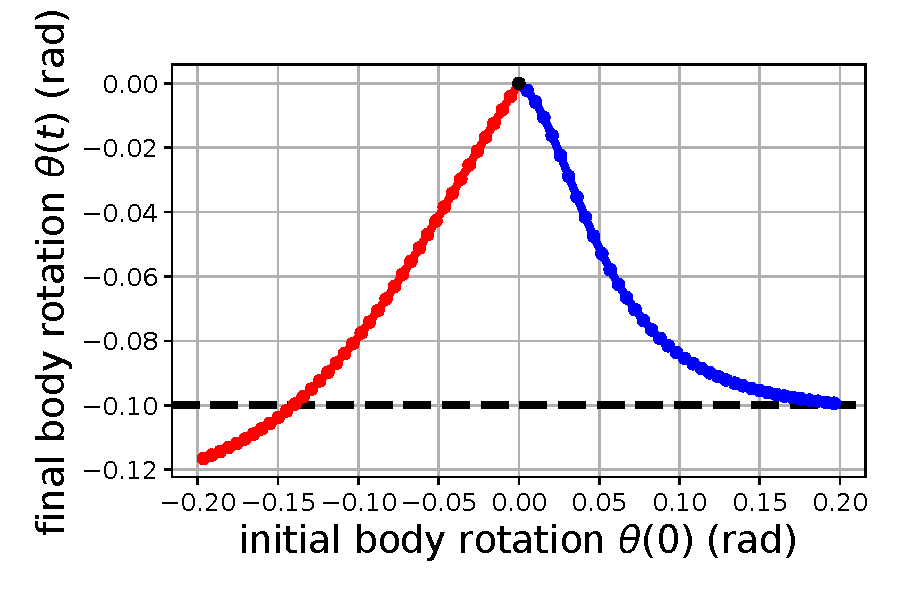
\includegraphics[width=.48\textwidth]{3a.pdf}
}
\subfigure[optimal liftoff trajectory outcomes]{
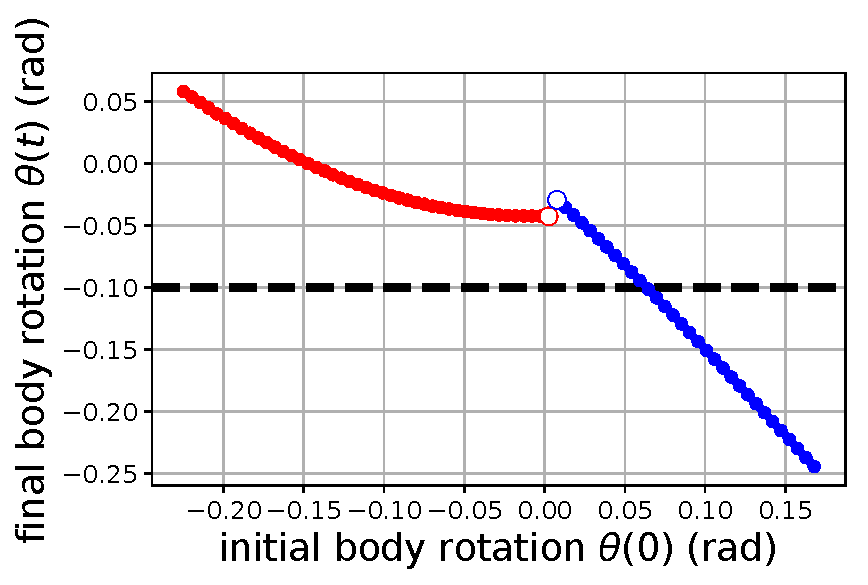
\includegraphics[width=.48\textwidth]{3b.pdf}
}

\subfigure[optimal touchdown policy]{
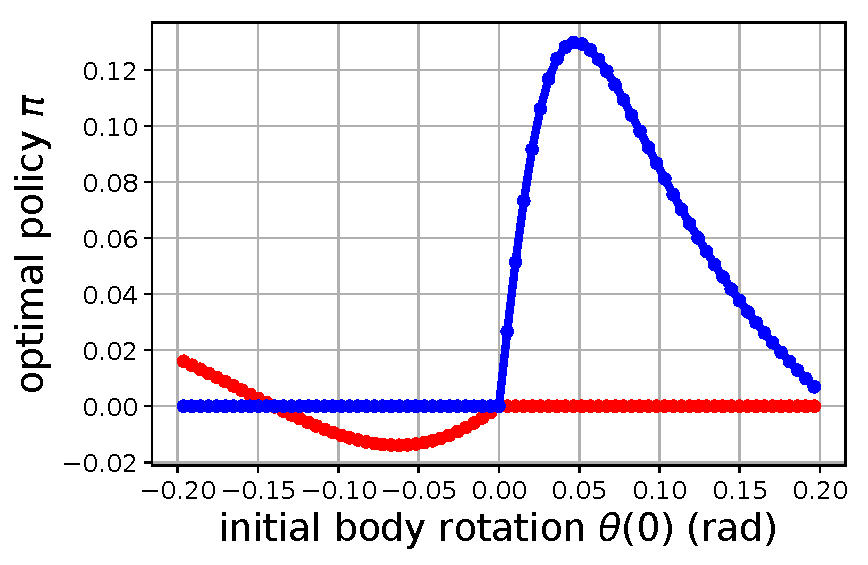
\includegraphics[width=.48\textwidth]{3c.pdf}
}
\subfigure[optimal liftoff policy]{
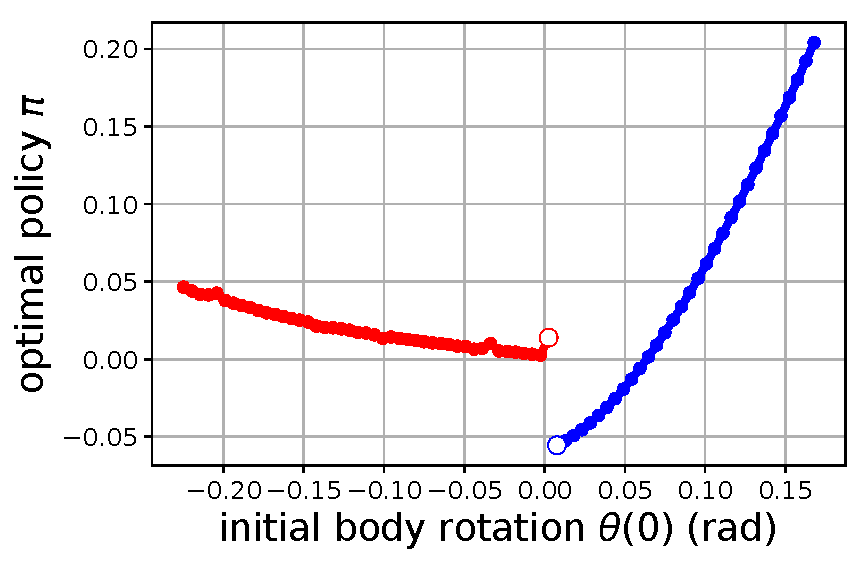
\includegraphics[width=.48\textwidth]{3d.pdf}
}

\subfigure[optimal touchdown value]{
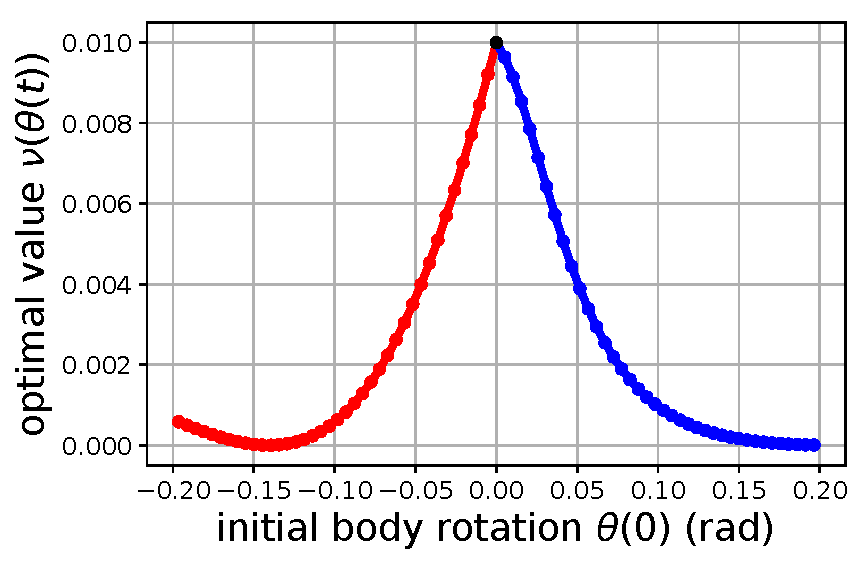
\includegraphics[width=.48\textwidth]{3e.pdf}
}
\subfigure[optimal liftoff value]{
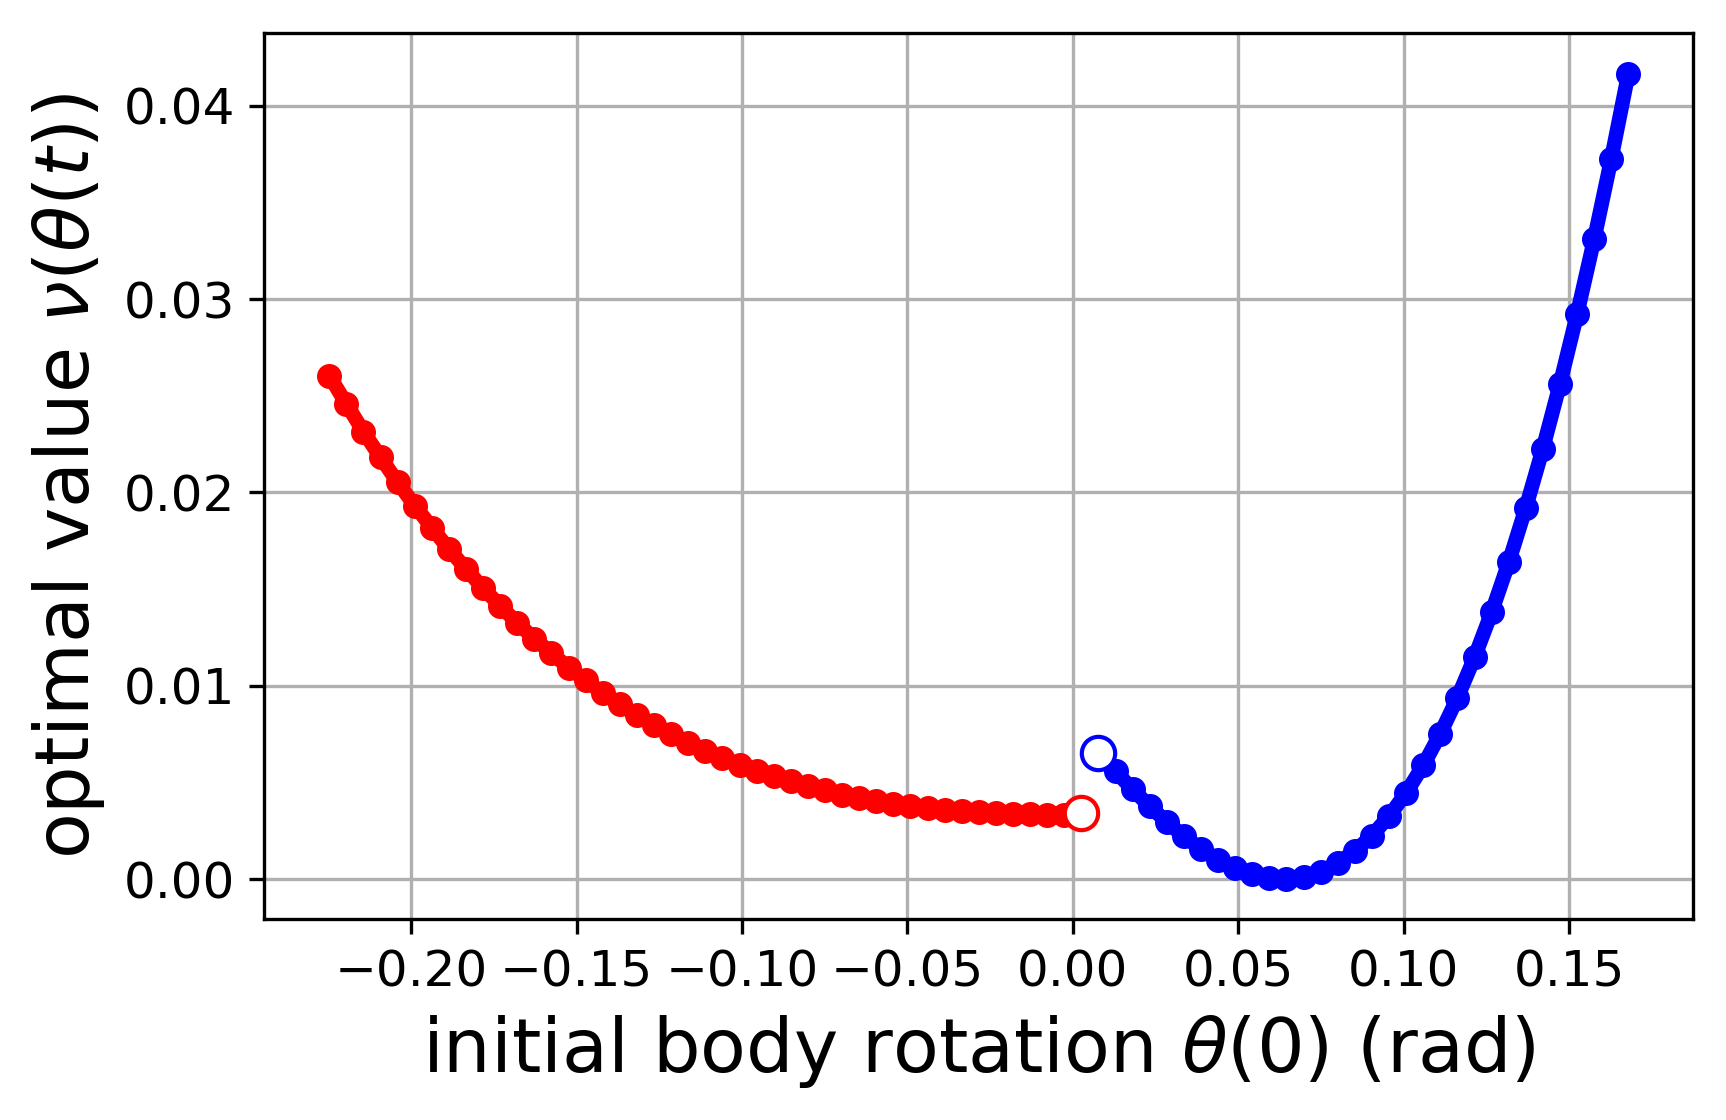
\includegraphics[width=.48\textwidth]{3f.png}
}

\caption{\label{fig:opt}
\emph{Optimal trajectories, values and policies for touchdown and liftoff maneuvers.}
Optimizing~\eqref{eq:touchdown:cost},~\eqref{eq:liftoff:cost} for the biped in~\figref{mdls} yields trajectory outcomes (a,b), policies (c,d), and values (e,f) that are nonsmooth (piecewise--differentiable or discontinuous).
%
%Illustrations of a simple mechanical system subject to unilateral constraints performing two distinct maneuvers under computed optimal policies. 
%(a) Smooth trajectory outcomes of the system performing the down maneuver.
%(b) Discontinuous trajectory outcomes of the system performing the up maneuver.
%(c) Smooth policy for the down system.
%(d) Smooth policy for the up the system.
%(e) Smooth cost function for the down system.
%(f) Smooth cost function for the up system.
}
\end{figure}


%==========

\section{Discussion}
\label{sec:disc}

We conclude by discussing
how often we expect to encounter the nonsmooth phenomena described above in models of robot behaviors (\secref{disc:models})
and
what our results imply about the use of smooth tools in this nonsmooth setting (\secref{disc:smooth}).


\subsection{Prevalence of nonsmooth phenomena near behaviors of interest}
\label{sec:disc:models}
In~\secref{opt}, we presented two simple optimal control problems where the dynamics of a mechanical system subject to unilateral constraints gave rise to a nonsmooth cost:
one where the cost was piecewise--differentiable,
and
another where it was discontinuous.
The reader may have noticed that the nonsmoothness manifested along trajectories that underwent simultaneous constraint (de)activation.
This peculiarity was not accidental:  
the cost is generally continuously--differentiable
along trajectories that (de)activate constraints at distinct instants in time.%
\footnote{This follows from~\cite[Eqn.~2.3]{Aizerman1958-ih} so long as the constraint (de)activations are \emph{admissible}~\cite[Def.~3,~Lem.~1]{Pace2017-tt}.}

If the constraint surfaces intersect transversely~\cite[Ch.~6]{Lee2012-mb},
then the nonsmoothness presented in~\secref{opt} is confined to a subset of the state space with zero (Lebesgue) measure. In light of this observation, intuition may lead one to ignore these states in practice. %
However, we believe this intuition will lead the practitioner astray as the complexity of considered behaviors increases.
%
Indeed, since the number of contact mode sequences increases 
factorially with the number of constraints
and 
exponentially with the number of constraint (de)activations,
then the region where the cost function is continuously--differentiable is ``carved up'' into a rapidly increasing number of disjoint ``pieces''
as behavioral complexity%
\footnote{as measured by the number of constraints and/or constraint (de)activations}
increases.

Although we cannot at present comment in general on how these smooth pieces fit together, we note that some important behaviors will reside near a large number of pieces.
For instance, periodic behaviors with (near--)simultaneous (de)activation of $n\in\N$ constraints as in~\cite{Alexander1984-ld} could yield up to $(n!)^k$ pieces after $k\in\N$ periods.
The combinatorics are similar for tasks that involve intermittently activating (a subset of) $n$ constraints $k$ times as in~\cite{Mordatch2012-ar}.
Since the dimension of the state space is independent of $n$ and $k$, these pieces must be increasingly tightly packed as $n$ and/or $k$ increase.


\subsection{Function approximation and gradient--based algorithms}
\label{sec:disc:smooth}

It is common practice to use smooth functions to approximate optimal value and policy functions.
This practice is justified for finite--state Markov Decision Processes (MDP) and smooth control systems whose value functions (optimal or otherwise) are known to be smooth under mild regularity conditions.
Our results imply that this practice is not generally justified for optimal control of mechanical systems subject to unilateral constraints since the value functions are generally discontinuous or only piecewise--differentiable. Future work could investigate the use of nonsmooth function approximators in this setting. 

Suppose a (possibly non--optimal) policy 
$\policy:\State\into\Inp$ 
has an associated value
$\val^\policy:\State\into\R$. 
If this value admits a first--order approximation with respect to $\policy$,
then it is natural%
%\footnote{If the norm in~\eqref{eq:algo:policy} is induced by the inner product with respect to the Hessian, this is a \emph{natural policy gradient}~\cite{Kakade2001-az}.}
~to improve the policy using steepest descent:
with $\alpha > 0$ as a stepsize parameter,
\eqnn{\label{eq:algo:policy}
\policy^+ = \policy + \alpha \arg\min_{\norm{\delta} = 1} \D_\policy\val^\policy(\delta).
}
The update in~\eqref{eq:algo:policy} is a \emph{direct policy gradient--based} algorithm~\cite{Sutton2000-ap, Baxter2001-ua}, and can be interpreted as a \emph{natural}~\cite{Kakade2001-az} or \emph{trust region}~\cite{Schulman2015-kr} algorithm depending on the norm chosen.
In practice, the derivative $\D_\policy\val^\policy$ is not generally available and must be estimated, e.g. using function approximation~\cite{Doya2000-gk, Konda2003-av} or sampling~\cite{Baxter2001-ua, Silver2014-lj}.
Analogously to the conclusions in the preceding paragraph, 
this practice is justified for classical systems (finite--state MDP, smooth control systems) whose value functions are smooth;
it is not generally justified for the systems considered here since the value of (optimal or non--optimal) policies can be nonsmooth.
It should be possible in future work to apply nonsmooth analogues of steepest descent~\eqref{eq:algo:policy} to these systems when the value function is piecewise--differentiable so that $\D_\policy\val^\policy$ is piecewise--linear.


Recent work employs smooth approximations of the contact--rich robot dynamics in~\eqref{eq:dyn} to enable application of gradient--based learning~\cite{Levine2014-im, Levine2016-lw, Kumar2016-nt} and optimization~\cite{Erez2012-yo, Mordatch2012-ar, Mordatch2015-jb} algorithms.
This approach leverages established scalable algorithms,
but does not guarantee that policies optimized for the smoothed dynamics will be (near--)optimal when applied to the original nonsmooth dynamics.
As an alternative approach, 
the framework recently introduced in~\cite{Pace2017-ph}
provides conditions under which the dynamics in~\eqref{eq:dyn} yield trajectories that depend continuously--differentiably on initial conditions.
Thus in future work it may be possible to justify applying established algorithms for optimal control directly on some mechanical systems subject to unilateral constraints.




\clearpage

\acknowledgments%
{This material is based upon work supported by the U. S. Army Research Laboratory and the U. S. Army Research Office under contract/grant number W911NF-16-1-0158.}

%===============================================================================

{%\small
\bibliography{refs}  % .bib
}

\end{document}
